\documentclass[tikz,border=8pt]{standalone}
% Shared look for every TikZ diagram. Load with \input{../../tools/tikz-style.tex}
\usepackage[T1]{fontenc}
\usepackage{lmodern}
\renewcommand{\sfdefault}{lmr}  % diagrams use the same serif as the text
\usetikzlibrary{arrows.meta, positioning, shapes.geometric, calc, fit, backgrounds}
\definecolor{cblue}{HTML}{4C78A8}
\definecolor{corange}{HTML}{F58518}
\definecolor{cgreen}{HTML}{54A24B}
\definecolor{cred}{HTML}{E45756}
\definecolor{cpurple}{HTML}{B279A2}
\definecolor{cgrey}{HTML}{6B6B6B}
\tikzset{
  every picture/.style={font=\sffamily, line width=1.2pt},
  box/.style={draw=#1, fill=#1!12, rounded corners=4pt, align=center, inner sep=7pt, minimum height=1.1cm},
  box/.default=cgrey,
  arrow/.style={-{Stealth[length=3mm]}, draw=cgrey, line width=1.4pt},
  title/.style={font=\sffamily\bfseries\Large},
  note/.style={font=\sffamily\small, text=cgrey, align=center},
}
\AtBeginDocument{\hyphenpenalty=10000 \exhyphenpenalty=10000}

\begin{document}
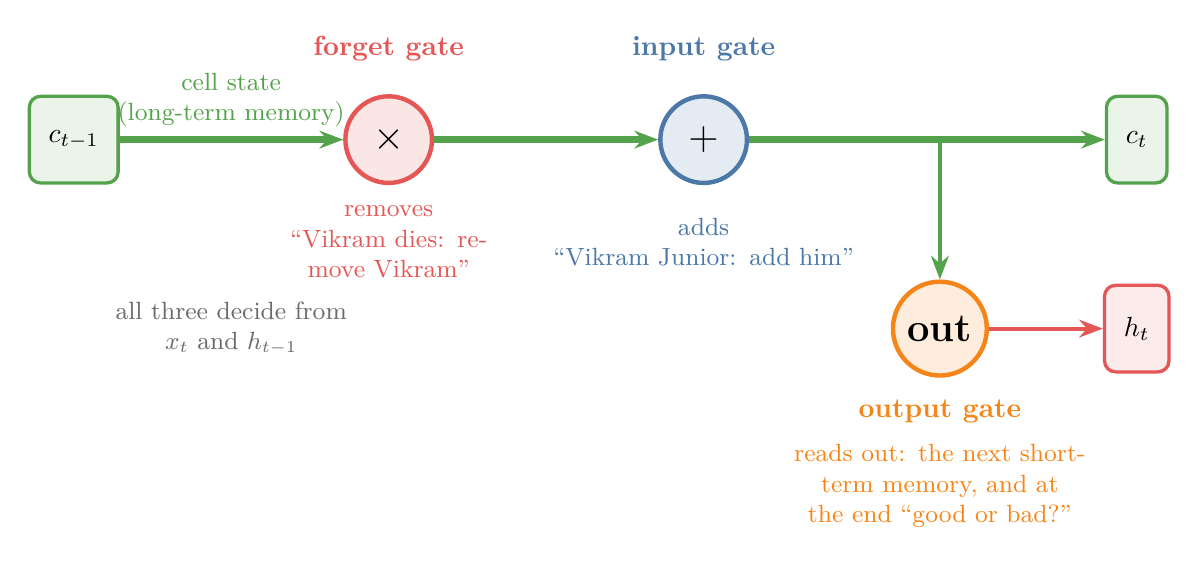
\begin{tikzpicture}[gate/.style={circle, draw=#1, fill=#1!15, line width=1.6pt, minimum size=1.1cm, font=\sffamily\Large\bfseries},
  ex/.style={note, text width=4.2cm}]
  \node[box=cgreen] (cin) at (0,0) {$c_{t-1}$};
  \node[gate=cred] (f) at (4,0) {$\times$};
  \node[gate=cblue] (i) at (8,0) {$+$};
  \node[box=cgreen] (cout) at (13.5,0) {$c_t$};
  \draw[arrow, draw=cgreen, line width=2.5pt] (cin) -- (f);
  \draw[arrow, draw=cgreen, line width=2.5pt] (f) -- (i);
  \draw[arrow, draw=cgreen, line width=2.5pt] (i) -- (cout);
  \node[note, text=cgreen] at (2,0.5) {cell state\\(long-term memory)};
  \node[gate=corange] (o) at (11,-2.4) {out};
  \draw[arrow, draw=cgreen] (11,0) -- (o);
  \node[box=cred] (h) at (13.5,-2.4) {$h_t$};
  \draw[arrow, draw=cred] (o) -- (h);
  \node[font=\sffamily\bfseries, text=cred] at (4,1.15) {forget gate};
  \node[font=\sffamily\bfseries, text=cblue] at (8,1.15) {input gate};
  \node[font=\sffamily\bfseries, text=corange] at (11,-3.45) {output gate};
  \node[ex, text=cred] at (4,-1.3) {removes\\``Vikram dies: remove Vikram''};
  \node[ex, text=cblue] at (8,-1.3) {adds\\``Vikram Junior: add him''};
  \node[ex, text=corange] at (11,-4.4) {reads out: the next short-term memory, and at the end ``good or bad?''};
  \node[note] at (2,-2.4) {all three decide from\\$x_t$ and $h_{t-1}$};
\end{tikzpicture}
\end{document}
